\documentclass[fleqn,useAMS,usenatbib]{mnras}
%=====================================================================
% CUSTOM: PACKAGES, MACROS & SETTINGS
%=====================================================================
% packages for figures
\usepackage{graphicx,todonotes}
% packages for symbols
\usepackage{latexsym,amssymb}
% AMS-LaTeX package for e.g. subequations
\usepackage{amsmath,morefloats}
\usepackage{natbib,graphicx,amsmath,subfigure,color}
\topmargin-1cm
\graphicspath{{figures/}}
\newcommand{\hmsun}{\ensuremath{h^{-1}M_{\odot}}}
\newcommand{\hgpc}{$h^{-1}$Gpc}
\newcommand{\hmpc}{$h^{-1}$Mpc}
\newcommand{\hkpc}{$h^{-1}$kpc}
\newcommand{\beq}{\begin{equation}}
\newcommand{\eeq}{\end{equation}}
\newcommand\notedo[1]{\todo[color=yellow, inline, size=\small]{To do:#1}}
\newcommand\notewrite[1]{\todo[color=orange, inline, size=\small]{To write: #1}}
\newcommand\noteask[1]{\todo[color=cyan, inline, size=\small]{To ask: #1}}
\newcommand\notecontrib[1]{\todo[color=green, inline, size=\small]{Contributors: #1}}
\newcommand{\vecM}{\mbox{\boldmath $M$}}
\newcommand{\vecg}{\mbox{\boldmath $g$}}
\newcommand{\vece}{\mbox{\boldmath $e$}}
\newcommand{\veck}{\mbox{\boldmath $k$}}
\newcommand{\vecQ}{\mbox{\boldmath $Q$}}
\newcommand{\vecF}{\mbox{\boldmath $F$}}
\newcommand{\vecD}{\mbox{\boldmath $D$}}
\newcommand{\matR}{\mbox{$\bf R$}}
\newcommand{\matC}{\mbox{$\bf C$}}
\newcommand{\bnab}{\boldsymbol{\nabla}}
\newcommand{\bnabg}{\boldsymbol{\nabla_g}}
\newcommand{\galsim}{\texttt{GALSIM}}
\newcommand{\ngmix}{\texttt{ngmix}}
\newcommand{\nnsim}{\texttt{nsim}}
\newcommand{\snr}{$S/N$}
\newcommand{\sn}{$S/N$}
\newcommand{\coadd}{{\rm coadd}}
\newcommand{\Msn}{$(S/N)_{\textrm{matched}}$}
\newcommand{\Tsn}{$(S/N)_{\textrm{size}}$}
\newcommand{\fsn}{$(S/N)_{\textrm{flux}}$}
\newcommand{\desreq}{$4\times 10^{-3}$}
\newcommand{\lsstreq}{$2\times 10^{-3}$}
\newcommand{\lognormscatt}{30}
\newcommand{\model}{\mbox{$\boldsymbol{m}$}}
\newcommand{\modelc}{\mbox{$\boldsymbol{m}_\coadd$}}
\newcommand{\comment}[1]{{\textcolor{cyan}{#1}}}

\newcommand{\mcal}{\textsc{metacalibration}}
\newcommand{\Mcalshort}{\textsc{metacal}}
\newcommand{\Mcal}{\textsc{Metacalibration}}
\newcommand{\vest}{\mbox{\boldmath $e$}}
\newcommand{\est}{e}
\newcommand{\mcalR}{\mbox{\boldmath $R$}}
\newcommand{\mcalRS}{\mbox{\boldmath $R_S$}}
\newcommand{\gest}{\mbox{\boldmath $\hat \gamma$}}
\newcommand{\vecgam}{\mbox{\boldmath $\gamma$}}

\title[The little coadd that could]{The little coadd that could:  Estimating shear from coadded images}

\author[Armstrong et~al.]{Bob Armstrong$^1$\thanks{\tt Bob's e-mail here}, Erin Sheldon$^2$, Eric
  Huff, Jim Bosch, Peter Melchior,
  \newauthor
  Rachel Mandelbaum, Robert Lupton
  \\$^1$Affil 1
  \\$^2$Affil 2
}

\begin{document}
\date{Draft \today}
\maketitle
% * <rearmstr@gmail.com> 2018-07-05T16:41:39.693Z:

\begin{abstract}
Upcoming wide field surveys will have many overlapping epochs of the same 
region of sky.  The conventional wisdom is that in order to reduce the 
systematic errors sufficiently for systematics limited measurements, like 
cosmic shear, we must do simultaneous fitting of all the epochs.  Using current 
algorithms this will require a significant amount of computing time and effort. 
In this paper, we examine the possibility of doing shear measurements on 
coadded images directly.  We show on a set of simulations that there is no bias 
or degradation in performance for two independent shear estimators.  The one 
caveat to working on coadds, is that we must remove images that overlap a CCD 
boundary, as the PSF is not well defined.  We estimate that the number of 
epochs that must be rejected for a survey like LSST is on the order of $\sim 3\%$.
\end{abstract}

\section{Introduction}
Future large scale astronomical surveys such as LSST \citep{LSST2009}, Euclid 
\citep{Laureijs2011}, and WFIRST \citep{Spergel2015} will gain an unprecedented 
increase in the combination of depth and area coverage.  Thus, enabling 
significant advances in many astronomical fields from the solar system to large 
scale cosmology.  The observing strategy for these surveys will repeatedly 
observe the same patch of sky in different filters.  The number of observations 
varies significantly between surveys and can range from only a handful to 
hundreds of exposures.  Having repeated visits helps to build up the required 
depth, fill-in chip gaps, and reject artifacts like cosmic rays.  Multiple 
observations can also help reduce systematic uncertainties, especially if they 
are taken on different parts of the camera.  One question that remains to be 
answered is, what is the optimal way to combine the information from these 
distinct sets of observations?  Past and current surveys have typically fallen 
into three categories:

\begin{enumerate}
\item \label{method:first} Resample all the images to a common pixel grid and 
take a weighted sum to construct a single coadded image.  Measurements are 
performed on the coadd with no need to return to the individual images.
\item \label{method:second} Perform measurements on each epoch separately.  
Combine these measurements by taking a weighted average.  
\item \label{method:third} Create the coadd as in \ref{method:first}, but only 
use the it to detect objects.  With this information, go back to each of the 
individual epochs and do a joint simultaneous measurement of all the images.
\end{enumerate}

The simplest option is \ref{method:first}, as it significantly reduces the 
complexity and computation time.  For a survey with many epochs this is a huge 
gain.  Many lensing surveys have chosen to work on coadded images 
\citep{Hoekstra2006, Leauthaud2007, Hettersheidt2007, Lin2012,Melchior2015, 
Jee2016, Mandelbaum2018}.  While this approach is attractive, it can also incur 
a number of problems if not done carefully.  First, we must ensure that the 
individual epochs are properly registered relative to another.  Mis-registered 
images can severely distort the shape of objects. Also, the PSF can be 
challenging to model on the coadd due to the fact that as you cross from the 
boundary of one detector to another there will discontinuous "jumps" in the 
shape and size of the PSF.  In addition, when combining images where the size 
of the PSF varies widely, there will be loss in S/N by doing a simple average.  
We discuss these problems in more detail in Section ~\ref{Section:Coaddition}.
Method \ref{method:second} has been used in fewer cases \citep{Jarvis2003}.  
The main problem with this approach is that there will be objects that do not 
have a large enough $S/N$ to be detected on any individual epoch, but will be 
detected on the coadd.  However, there has been some work recently on how one 
might do this \citep{Budavari2017}.

With the need to reduce systematic errors, a number of recent surveys have 
followed the hybrid method \ref{method:third}.  The CFHTLens 
\citep{Heymans2013} and KIDS \citep{Hildebrandt2017} collaborations performed 
photometry and detection on the coadds and shear measurements via multi-epoch 
fitting. For the Dark Energy Survey (DES) \citep{Zuntz2017}, only object 
detection was done on the coadd and all other measurements were performed on 
individual epochs.  This approach has worked well to reduce the systematic 
errors sufficiently low for cosmological analyses.  Can this multi-epoch 
fitting approach be applied to future surveys as well?
As the number of exposures increases, the computational demand scales as well.  
Existing surveys typically have fewer than $\sim10$ epochs to fit 
simultaneously. For a survey like LSST, where the number of epochs is an order 
of magnitude larger, it is likely that multi-epoch fitting will overwhelm the 
computing budget.  Again, being able to instead work on a single coadd could 
reduce a significant amount of the processing burden.  There may also be other 
reasons to prefer working on the coadds.  When separating blended objects into 
their individual sources, there is limited information available on single 
epochs.  The higher $S/N$ on the coadds makes this much easier.  

In this paper, we explore the possibility of avoiding multi-epoch fitting by 
demonstrating that we can recover shear on coadds without incurring systematic 
errors.  In Section \ref{Section:Coaddition}, we discuss the problems using 
coadds and potential ways to mitigate them.  We propose to create per object 
coadds of the image, PSF and the noise.  We test this proposal by looking at 
the measured shear bias on simulations of both multi-epoch and coadd data.  
Section \ref{Section:Simulation} describes the setup and properties of the 
simulations.  We test two separate shear measurement pipelines: BFD and 
\Mcal.  We summarize how these algorithms were configured and applied 
in Section \ref{Section:Measurement}.  Section \ref{Section:Results} shows the 
results of these methods.  We show that for both shear methods, we are able to 
recover unbiased results.  The advantage of running more than one algorithm 
shows that our results are not specific to a particular shear estimator, but 
are more generally applicable.   Finally, in Section ~\ref{Section:Exclusion} 
we look at the cost of rejecting images from our coadds for the specific case 
of LSST.

\section{Coaddition}
\label{Section:Coaddition}
The simplest means of combining images is to use a median, weighted mean or 
clipped mean.  None of these are optimal in $S/N$ because they do not properly 
account for variations in PSF sizes and background levels.  For the majority of 
detections, which are small faint objects, the epochs with the smallest seeing 
will have the most information.  \cite{Kaiser2004,Zackay2017} proposed 
constructing an optimal coadd, by stacking the image convolved with the PSF.  
This results in an image that loses no information when combining epochs of 
different seeing.  Further research in this area seems promising in order to 
maximize the $S/N$ for a coadd.  However, for this paper we only consider the 
scenario of using a simple weighted mean.  

\subsection{Image Registration and Noise}
\label{Subsection:Registration}
%\begin{figure*}
\begin{figure}
%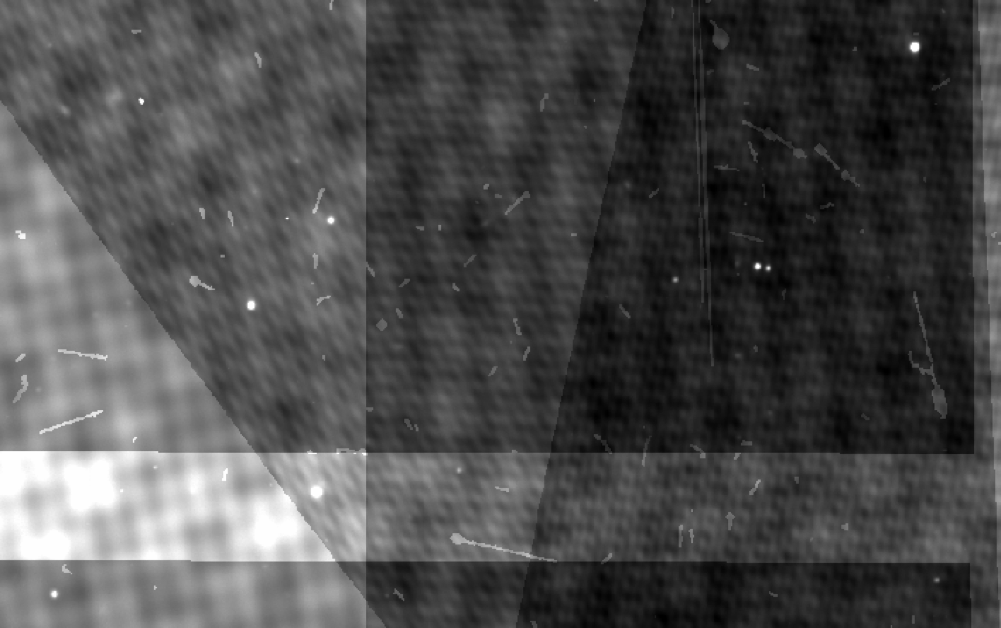
\includegraphics[width=0.65\textwidth]{CoaddNoise.png}
%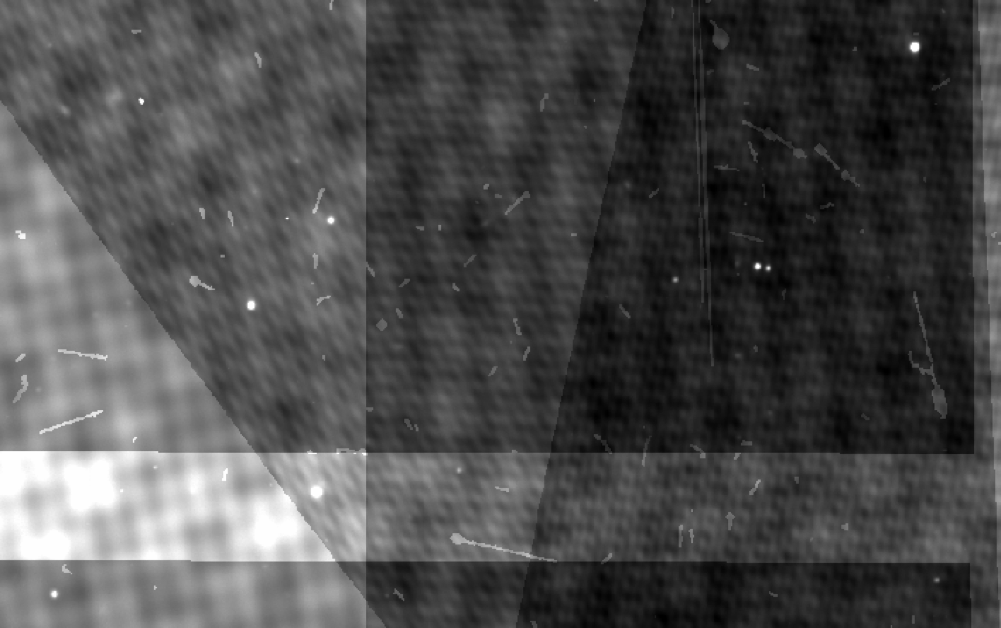
\includegraphics[width=\columnwidth]{CoaddNoise.png}
\caption{
The variance map from a random location from the HSC DR1 survey.  Darker colors 
indicate lower variance or a larger number of visits.  This map is constructed 
by coadding all the variance maps of the individual epochs.
}
\label{fig:noise}
\end{figure}
%\end{figure*}

In order to coadd, we must account for the actual pointing of each image and 
the local distortion caused by the optics, atmosphere, etc.  This requires 
resampling and interpolating each image onto the same coordinate grid.  This 
interpolation will cause the noise in the image to have correlations from pixel 
to pixel.  In addition, depending on the local distortion and relative offset 
between pixel grids, this can cause the noise to become non-stationary, i.e. it 
can vary over the size of the image.  Figure \ref{fig:noise} shows a pixel 
variance map of the coadded image from a random position in the HSC survey 
\cite{HSC_DR1} from their first data release.  The image cutout corresponds to 
a region roughly $3\arcmin \times 1.5\arcmin$ in area.  The darker regions have 
more observations and hence lower variance.  The large slices seen correspond 
to edges of individual CCDs.  Also visible are the small scale variations 
resulting from resampling and grid offsets.  The streaks correspond to cosmic 
rays that are masked on individual epochs.  The range of variations is 
$\sim10\%$ and the scale on which they vary is close to the average size of on 
object (see \ref{Section:Exclusion}).

By definition, the variance map does not include the pixel to pixel covariance. 
This will also vary spatially depending on the dither pattern and 
interpolation kernel.  For typical observing patterns in HSC, the amount of 
variance lost to covariance is $~10\%$.  The correlated noise pattern must be 
taken into account to achieve the precision in weak lensing. \cite{Gurvich2016} 
showed that ignoring such correlations results in errors of a few percent, well 
above the requirements.  

With a complete knowledge of the astrometric shifts and distortions, it is, in 
principle, possible to construct the full pixel covariance for a given region.  
However this is far from practical and few algorithms currently would be able 
to take advantage of such information.  As an alternative, we propose to take 
Monte Carlo realizations of the noise for each epoch and coadd them in the same 
way as the image.  The resulting coadded noise image can then be used to 
account for the correlations. 

\subsection{PSF}
\label{Subsection:PSF}
In many situations, we need to be able to model the PSF from the observed stars 
and interpolate it to the positions of galaxies.  Typically, a low order 
polynomial is used to describe the variation of the PSF across a CCD.  The 
challenge on a coadd is that you have sharp changes whenever you cross the edge 
of a detector in any epoch.  Given this, it can be difficult to construct a 
model on the coadd.  An alternative approach used by 
\cite{Jee2016,Mandelbaum2018} is to create a valid coadded PSF by resampling 
and interpolating the single epoch PSFs in the same way as the images 
\cite(DLS, HSC).  This avoids any problems of having to spatially interpolate a 
complex PSF model.  However, objects that include an epoch which crosses a 
detector boundary will pose a problem ,as the PSF is not be well defined.  For 
HSC DR1, objects that contained such a boundary image were flagged and 
corresponded to $\sim15\%$ of the detected objects.  Because the PSF is 
potentially inaccurate, these objects should be removed from scientific 
analyses.  This will not be a viable option for a survey like LSST, as almost 
every object will cross at least one CCD boundary.  Instead of flagging these 
objects, we propose to simply throw out epochs that cross a detector boundary 
when creating the coadd.  This means we can no longer construct a unique coadd 
for all objects, as each object will need to potentially reject different 
epochs.  But the advantage is that the coadded PSF model can be correctly 
reconstructed.  We discuss the loss of depth from rejecting these visits in 
\ref{Section:Exclusion}.

\subsection{Expected Flux $S/N$ loss}
\label{Subsection:FluxSN}


For the simple weighted mean coadds used in this work, we expect measurements
on a coadd to be noisier than those using optimal multi-epoch fitting when the
size of the PSF varies between epochs.  We expect the increase in noise to be
largest for the smallest objects such as stars and distant galaxies, the images
of which are more affected by the PSF.

To gain some intuition, we derive the functional form of the expected loss in
$S/N$ for the case of a linear fit for the amplitide $A$ of a template, or
``matched filter''.  In this case we can analytically compute the uncertainty
in the estimated flux, $\hat{A}$, from a linear fit to the data (see Appendix
\ref{Subsection:FluxSN}). It is also useful to introduce a ``toy model'', which
illustrates the main features of this process.  For the toy model we use data
that follows a circular Gaussian, which makes the calculations easier and
allows introduction of useful approximations.

In Appendix \ref{Subsection:FluxSN} we show that, for the toy model and small
variations in the PSF size, the ratio of the flux variance derived from the
coadd to that from fitting the epochs simultaneously is approximately:
\begin{align} \label{eq:vargal}
\left( \frac{ {\rm var} \hat{A}_\coadd}{{\rm var} \hat{A}_{\rm multi} } 
\right) &
\approx 1 + 2 \left( 1 - R \right)^2 \left( \frac{\Delta 
\sigma_p}{\sigma_p} \right)^2,
\end{align}
where $\sigma_p$ is the PSF size, $\Delta \sigma_p$ is the RMS scatter in PSF
size, and $R=\sigma_g^2/(\sigma_p^2 + \sigma_g^2)$ is the ratio of the galaxy
size, $\sigma_g$, to the PSF size.  This result shows the increased variance is
proportional to the resolution, $R$, and the relative variation in PSF size
$(\Delta \sigma_p/\sigma_p)^2$.  For a large galaxy $R$ is near unity and for a star
$R$ is near zero, so as expected the effect is largest for stars.  In cases where there
are significant PSF variations of order 1, the variance could be increased by a
factor of 2 or three for star-like objects.  However, most current and future
surveys have significantly less PSF variation than this, on the order of 0.1.

We tested the validity of equation \ref{eq:vargal} using a simple Monte Carlo
simulation.  We used the \galsim\ package to generate images of Gaussian
galaxies, convolved by Gaussian PSFs, and used the \ngmix\ package
\footnote{\url{https://github.com/esheldon/ngmix}} to fit for the flux. We used
a PSF with FWHM=0.9 arcsec, with Gaussian variation between images of $\Delta
\sigma_p/\sigma_p = 0.1$.

All images were placed at the center of the image, so that no interpolation was 
required when coadding the images.  We used the same constant noise for all 
images, and used a simple mean for the coaddition process.  The primary 
variable of interest is the resolution $R$.  We varied the size of the galaxy 
from zero, or star-like, to more than twice the PSF size, such that $<R> = 
0.83$.  A comparison of the results from the simulations and analytical formula 
are shown in Figure \ref{fig:mcresults}.  The points are the measured values 
and the solid line are the exact variance estimators from 
\ref{eq:exact_var_coadd} and \ref{eq:exact_var_mult}.  The dotted lines are the 
predicted values from the toy model in equation \ref{eq:vargal}.  We can 
see that the toy model slightly over-predicts the increase in variance, but is 
still evidently useful for understanding how the effect scales with resolution. 
For a given survey we can use this to predict the effect that coaddition will 
have on the flux uncertainty.  For current and future surveys the effect seems 
to be quite small, especially for galaxys.

\begin{figure}
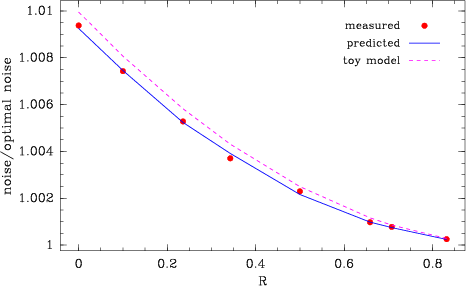
\includegraphics[width=0.45\textwidth]{toy-model.png}
\caption{Measured and predicted values for the increased uncertainty due to 
coaddition, for the Gaussian galaxies and stars.  The points are the measured 
values from simulations, and the solid line is the exact prediction from 
equations in Appendex \ref{Section:FluxSN}.  The dashed line shows the simple 
toy model presented in equation \ref{eq:vargal}.}
\label{fig:mcresults}
\end{figure}

\section{Simulations}
\label{Section:Simulation}
While the insight derived in the previous section was instructive, there are 
many potential complications in real data that could make things harder when 
measuring shear.  Therefore, we construct a suite of simulations to test the 
impact of coaddition specifically for shear estimators.  The goal is to 
simulate multiple epochs of the same galaxy with a known shear and compare the 
measured shear from both a multi-epoch approach and when coadding the epochs 
together.  The observing conditions for each epoch (noise, PSF, etc.) are 
simulated to roughly match observations from DES data.  While DES will have 
only ten epochs by the end of the survey, it still provides a useful test while 
reducing somewhat the computation time.  Even with 10 epochs, the computation 
time to generate the dataset is significant as we need to simulate billions of 
galaxies to reach the needed precision for cosmic shear.  With fewer epochs, we 
may also be more sensitive to certain systematic errors that could get averaged 
down for a survey with many more observations.
To generate the galaxy population we use code from the \nnsim\ package 
\footnote{\url{https://github.com/esheldon/nsim}} which is based on \galsim\ 
and \ngmix\.  The generated galaxy images have the following properties:

\begin{itemize}
\item We generate single galaxy images on 48x48 postage stamps with no 
neighbors.
\item The pixel noise is uniform for each visit and is modeled as a zero-mean 
Gaussian with $\sigma$ ranging from 0.5-0.6.
\item Assume the PSF model is perfectly known.
\item The PSF model is a Moffat with $\beta=3.5$.
\item The \textsf{FWHM} of the PSF varies for each epoch as a Log-Normal 
distribution with mean 0.95 and $\sigma=0.1$ 0.1.  Values are truncated between 
0.8 and 1.15.
\item The PSF ellipticity is Gaussian with a mean of 0.0 and 0.01 for $e_1$ and 
$e_2$ respectively, and $\sigma=0.01$.
\item The galaxy models are pure exponentials.  
\item We sample from an empirical model for the flux and size based on 
\textsf{COSMOS} data.  We used the \textsf{COSMOS} data packaged along with the 
\galsim\ software to construct a kernel density estimator for the size and 
flux.  For the bandwith of the estimator we usea kernel with 0.1$\times$ the 
intrinsic data covariance.  
\item The intrinsic ellipticity is drawn from the distribution $P(e) \propto 
(-e^2)^2 \rm{exp}(-e^2/2\sigma_e^2)$ with $\sigma=0.02$.
\item We generate 10 epochs for each object.  
\item Each visit has a random shift applied within a 0.5 pixel radius.
\item The Jacobian values of the WCS for each exposure are allowed to vary for 
each epoch.  The amount of variation is taken from values measured on DES.
\item To resample the images we use a 3rd order Lanczos kernel.
\item For coaddition, we compute a mean weighted by the inverse of the pixel 
variance.
\item We construct a coadded noise image, as described in 
\ref{Subsection:Registration}, by generating a single Monte Carlo realization 
of the noise for each epoch and resampling and coadding them.
\item The coadded PSF is constructed by resampling and coadding the individual 
PSFs for each epoch.
\item All galaxies are sheared by $g_1=0.02$.
\end{itemize}

The choice of using simplified galaxy models was employed solely to reduce the 
computational run time.  For more complicated models there was significant 
computation time in generating the images.  We did some limited testing of more 
complicated galaxy models with reduced statistics, and these showed no sign of 
problems.  Since both of the shear measurement pipelines employed here have 
already shown to be largely insensitive to the type of galaxy model chosen, we 
do not expect this to affect our results.

\section{Measurement Methods}
\label{Section:Measurement}
We employ two different algorithms to measure the applied shear.  We briefly 
summarize these methods and describe how they were applied for these 
simulations.

\subsection{BFD}
\label{Section:BFD}
The Bayesian Fourier Domain (BFD) method \citep{Bernstein2014,Bernstein2016} 
was designed to overcome some of the inherent biases that arise from the 
measurement of galaxy shapes.  It relies on measuring the distribution of 
intensity-weighted moments in Fourier space.  It requires knowledge of the true 
intrinsic distribution of these moments, which we call the prior, and their 
derivatives with respect to shear.  We can use observations of a deeper dataset 
to approximate the true prior distribution.  Most ongoing and future large 
surveys contain a smaller, deeper component suitable for this purpose.  Given 
that we are computing moments with a fixed weight function, the moments and 
their derivatives can be computed analytically for each galaxy.  
As noted in \citep{Bernstein2016}, because the BFD moments are linear, 
measurements on multiple exposures can be combined at the catalog level by 
taking weighted sums of the individual moments.  This is true as long as each 
individual exposure is unaliased.  This greatly simplifies doing a 
muli-exposure measurement compared to other methods because there is no need to 
go back to the individual pixels.  
For the coadd we need to have an accurate measure of the pixel noise power 
spectrum.  We can measure this directly from the coadded noise image for each 
object.
We configure the BFD code to run with the following parameters:

\begin{itemize}
\item We use the '$k\sigma$' weight function as defined in \cite{Bernstein2016} 
Section 3.3.  The parameters are set to $N=4$ and $\sigma=1$.  We chose 
$\sigma$ to be slightly smaller here because it avoids the small bias seen in 
image simulations.  Other parameters were chosen to match those listed in the 
\galsim\ settings from Table 1 in \cite{Bernstein2016}.
\item We simulated a deep dataset with the same settings, except the pixel 
noise was reduced by a factor of 100.
\item We divide the data into two different regimes: $S/N$ 5-25 and 25-50.  We 
build a separate prior for each dataset.  For the higher range, we doubled 
measured moment noise to increase the overlap with the number of deep galaxies.
\item A knowledge of the covariance matrix is currently necessary in order to 
build the prior moment distribution.  Previous studies have shown that if the 
noise varies more than $\sim 10\%$, we need to divide the data into different 
samples and construct a separate prior for each sample.  In this case, we saw 
that the variation in covariance was sufficiently small that we only needed to 
construct a single prior.
\item The single epoch moments were weighted by the inverse variance of the 
flux moment when combined for the multi-epoch measurement.  
\end{itemize}

\subsection{\Mcal}
\label{Section:Metacal}

\Mcal\ is a method to calibrate weak lensing shear measurements using
transformations of the real images, without reference to external data sets or
simulations \citep{HuffMand2017,SheldonHuff2017}.  Below we give a brief review
of the \mcal\ formalism.  For full details of the method used in this work, see
\cite{SheldonHuff2017}.

The basic assumption behind \mcal\ is that the two component shear estimator \vest\
is linearly related to the applied shear $\vecgam$, such that
\begin{align} \label{eq:Eexpand}
    \vest &= \vest|_{\gamma=0} + \frac{ \partial \vest }{ \partial \vecgam}\bigg|_{\gamma=0} \vecgam  + ... \nonumber \\
          &\equiv \vest|_{\gamma=0} + \mbox{\mcalR}\vecgam  + ...
\end{align}
We have defined the $2 \times 2$ shear response matrix
\begin{align}
    \mbox{\mcalR} &\equiv \frac{\partial \vest}{\partial \vecgam} \bigg|_{\gamma=0}.
\end{align}
With \mcal\ these derivative are performed by shearing the real image
of the object and calculating a finite difference derivative.  The image
is deconvolved from the PSF, sheared by a small amount, and reconvolved by
a larger PSF to suppress amplfied noise.  Measurements $\vest$ are then made
on these images and the derivatives are formed. For element $i,j$
\begin{equation} \label{eq:Rnum}
    R_{i,j} = \frac{\est_i^+ - \est_i^-}{\Delta \gamma_j}.
\end{equation}

For the measurement of simple mean shear, which is all we will  use in this
work, the calibrated estimator is formed using the ensemble mean of the
estimator and response
\begin{align}
    \langle \vest \rangle &= \langle \vest \rangle |_{\gamma=0} + \langle \mbox{\mcalR} \vecgam \rangle + ... \nonumber \\
                          &\approx \langle \mbox{\mcalR} \vecgam \rangle,
\end{align}
and thus
\begin{align} \label{eq:rcorr}
    \langle \gest \rangle &= \langle \mbox{\mcalR} \rangle^{-1}  \langle \vest \rangle \approx \langle \mbox{\mcalR} \rangle^{-1} \langle \mcalR \vecgam \rangle.
\end{align}

Note that if selections are performed on the measurements, an additional
response \mcalRS\ must be calculated and added to the ensemble response
to correct for shear-dependent selection effects \citep{SheldonHuff2017}.

The convolutions and shears applied to the images result in correlated noise
that can bias the shear estimate. We apply a simple empirical correction. We
generate a noise image with the same amplitude as the noise in the real data,
and the same shape as original image.  We rotate the noise image by 90 degrees.
We apply \mcal\ shearing and convolution operations.  We then rotate this field
back by 90 degrees and add it to the image of the object before performing a
measurement. This cancels the correlated noise bias in the ensemble shear
measurement \citep{SheldonHuff2017}.

Coaddition involves interpolation of the images, which introduces additional
correlated noise.  This can be dealt with in the same correlated noise
correction scheme.  We generate noise images as described above, but pass them
through coaddition before passing them through the convolution and shearing
operations.


\section{Simulation Results}
\label{Section:Results}

\subsection{Shear bias} We ran the BFD and \mcal\ shear measurement codes on
our simulations in both multi-epoch measurements and on the coadded images. For
\mcal\ we made cuts that the object have \snr$ > 10$ and square size relative
to the PSF of $T/T_{\mathrm{PSF}} > 0.5$.  For BFD we made cuts XXX.  We
applied corrections for selection effects in both methods.  We summarize the
results in table \ref{tab:results}.  Each measurement was performed on
independent simulations, so the errors are uncorrelated.  These results show
that there is no additional bias in either shear method when measuring the
shear on the coadds.  We note additional findings from our
analysis: 

\begin{itemize}

\item The Monte Carlo noise images that we generated for each epoch were the
same size as the galaxy postage stamp; 48 by 48 pixels.  If the size of the
noise image is reduced we see a bias in the BFD results.  Reducing the noise
image to 40 by 40 results in a $\sim 1\%$ bias and increases as you decrease
the size.  Presumably, this comes from not having sufficient information to
construct the power spectrum accurately on the final coadd.  Note \mcal\
has a strict requirement that noise image must be at least as large as the
original image.

\item Initially, \mcal\ required a very high order interpolation kernel (order
15) to remove a bias of a few percent in the shear.  We believe this came from
noisy interpolations that caused a ``smearing'' of the image.  This smearing
was different from that present in the PSF image, as the PSFs were initially
centered in the middle of the postage stamp.  If instead we offset the PSFs so
that it was interpolated in the same way as the object images during
coaddition, we found that the bias went away and we could use a lower order
interpolation kernel.  This problem did not seem to effect the BFD method.
This is likely because in BFD we making the same error in the deep reference
set as in the shallow images, so this problem was being calibrated out.

\item We tested coadds created from original images that had large random
rotations.  We found no additional bias, as long as the images were padded
sufficiently to avoid corner effects.

\end{itemize}

\begin{table}
\begin{tabular}{ll}
\hline
Sample & Measured bias \\ \hline
BFD Coadd & $0.0012 \pm 0.0007$ \\
BFD Multi-epoch & $-0.0014 \pm 0.0007$ \\
\mcal\ Coadd & $0.0007 \pm 0.0004$  \\
\mcal\ Multi-epoch & $0.0004 \pm 0.0004$  \\ \hline
\end{tabular}
\caption{The measured shear bias from simulations for BFD and \mcal\ on both 
coadd and multi-epoch data.  These results show no statistically significant 
bias for any of the methods beyond that expected from the breakdown
of the weak shear approximation ($\sim 0.0005$).}
\label{tab:results}
\end{table}

\subsection{Shear S/N}
We computed the S/N for both the multi-epoch and coadd cases to test if there 
was any loss in $S/N$ on the measured shear.  BFD saw no loss in $S/N$, while 
\mcal\ saw a small effect of order 0.5$\%$.

\section{S/N Loss from Rejecting Exposures}
\label{Section:Exclusion}
As mentioned above, in order to build a per-object coadd we must reject 
exposures where the edge of a CCD overlaps the object.  This will result in 
some loss of information from these rejected exposures.  We estimate how many 
exposures would be rejected for a typical object using a simulation of the LSST 
survey as described in \cite{LSSTSims}.  This simulation gives a nominal 
pointing for each exposure of the 10-year LSST survey.  We used the the 
baseline \textsc{OpSim} catalog \textsf{minion\_1016} to define the camera 
pointings.  By default the simulation does not provide a dithering strategy for 
different exposures of the same pointing.  Since the final dithering strategy 
is still under discussion in LSST, this gives us the option to try different 
strategies and test different metrics for difference science cases.  Therefore, 
we implemented a number of different dither strategies as provided by the LSST 
Metrics Analysis Framework (MAF) software \citep{LSSTSims}.  We found that the 
results had little dependence on which dithering strategy was chosen, therefore 
we will only show two representative dither patterns - a random offset for each 
visit and a spiral pattern. Fig.~\ref{fig:dither} shows the distribution of 
offsets for these two patterns.

\begin{figure}
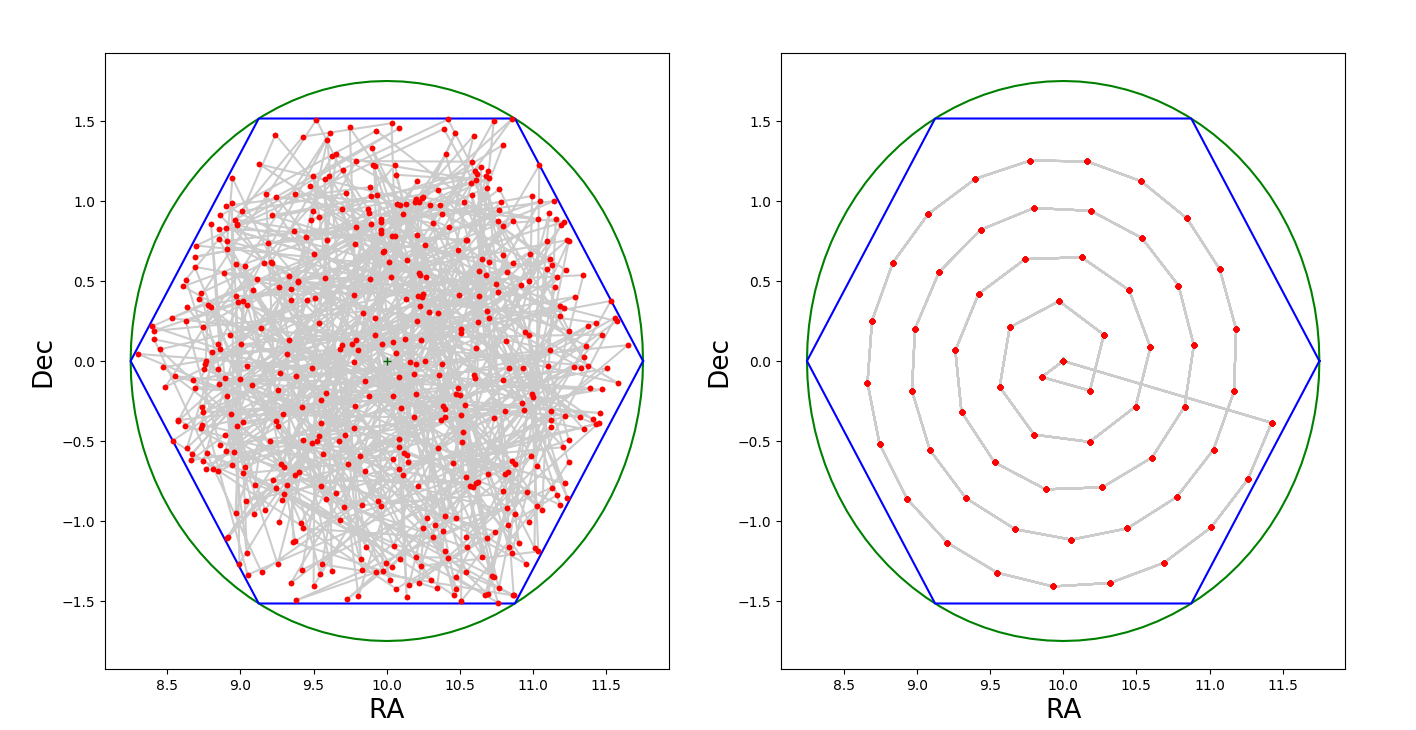
\includegraphics[width=0.5\textwidth]{Dither.png}
\caption{
Two different LSST dither patterns are show.  On the left each visit gets a 
random position and on the right a spiral pattern.  The green circle represents 
the approximate size of the LSST focal plane.  Each dot shows a separate offset 
from the nominal pointing.  The dots are restricted to within the blue hexagon 
for this study.
}
\label{fig:dither}
\end{figure}

To compute the number of missing exposures we might expect, we place 10,000 
square patches of a particular size on the sky and calculate the number of 
visits that have a CCD edge that will cross each patch.  We can also calculate 
the reduced 5$\sigma$ point source depth for each patch.  Fig.~\ref{fig:dither} 
shows these values for three different patch sizes with side length 0.1, 0.5 
and 0.8 arcminutes. Given these patch sizes, the fraction of rejected visits 
can vary from 3$\%$ to 20$\%$.  This emphasizes the fact that we must use small 
patches to avoid losing many visits.  
To connect this with observations we need to know the typical object size in 
LSST.  In Fig.~\ref{fig:size}, we show the distribution of blend family sizes 
from the HSC Ultra-Deep\citep{SurveyOverview} data.  The HSC Ultra-Deep data is 
a good match for LSST because it has a depth of $\sim27.5$ which is comparable 
to the wide field LSST depth.  Note that this is not the size of single 
objects, but rather the size of objects that have been identified as coming 
from the same blend.  A blend is defined as objects that have been combined 
because contiguous pixels above threshold overlap.  The LSST software is fairly 
loose in combining nearby structures as it is fairly easy to "deblend" objects 
at large separations.  
The blend sizes are computed from the bounding box of the above threshold 
pixels.  We use the square root of the area of the bounding box as a proxy for 
its size.  From the figure we can see that most objects have box sides of 
$~\sim 0.05$ which corresponds well with our patch side of 0.1 arcminutes.  We 
therefore conclude that a typical object therefore, will only suffer a small 
decrease in $S/N$ by rejecting visits that cross a CCD boundary.

%\begin{figure*}
\begin{figure}
%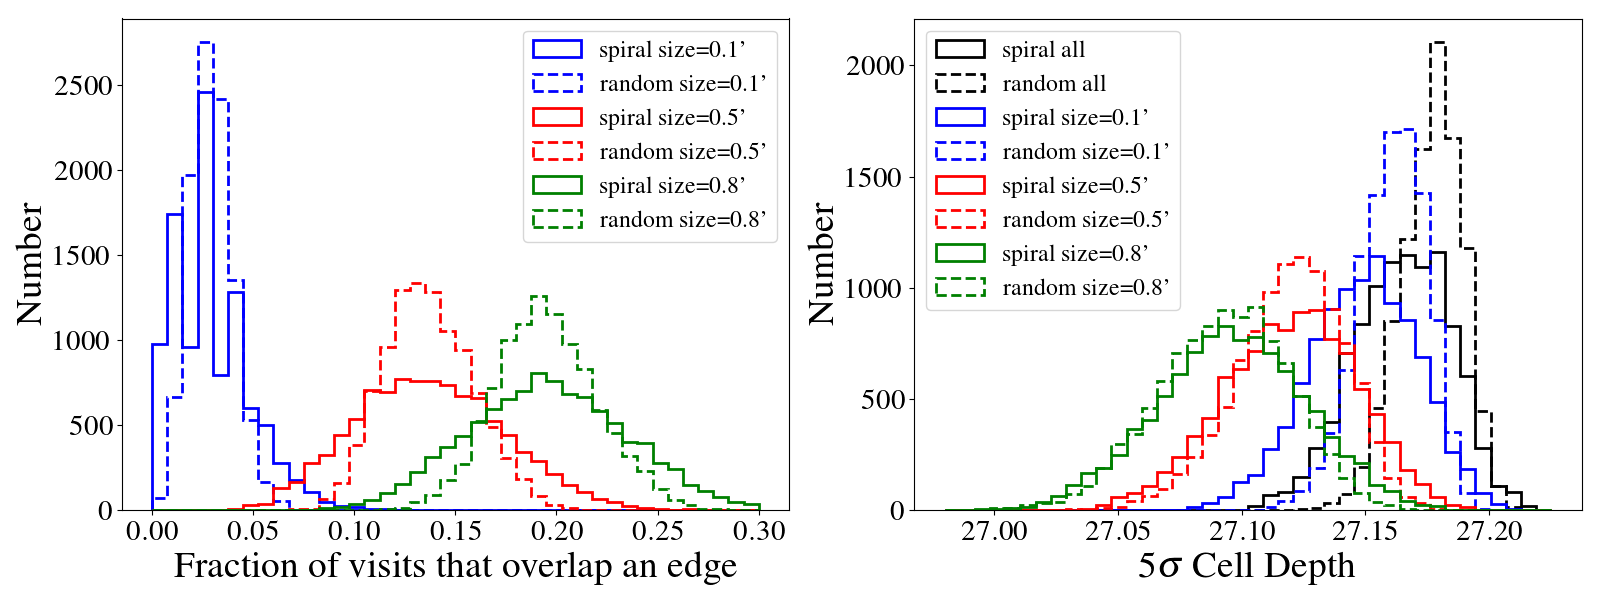
\includegraphics[width=0.8\textwidth]{cell.png}
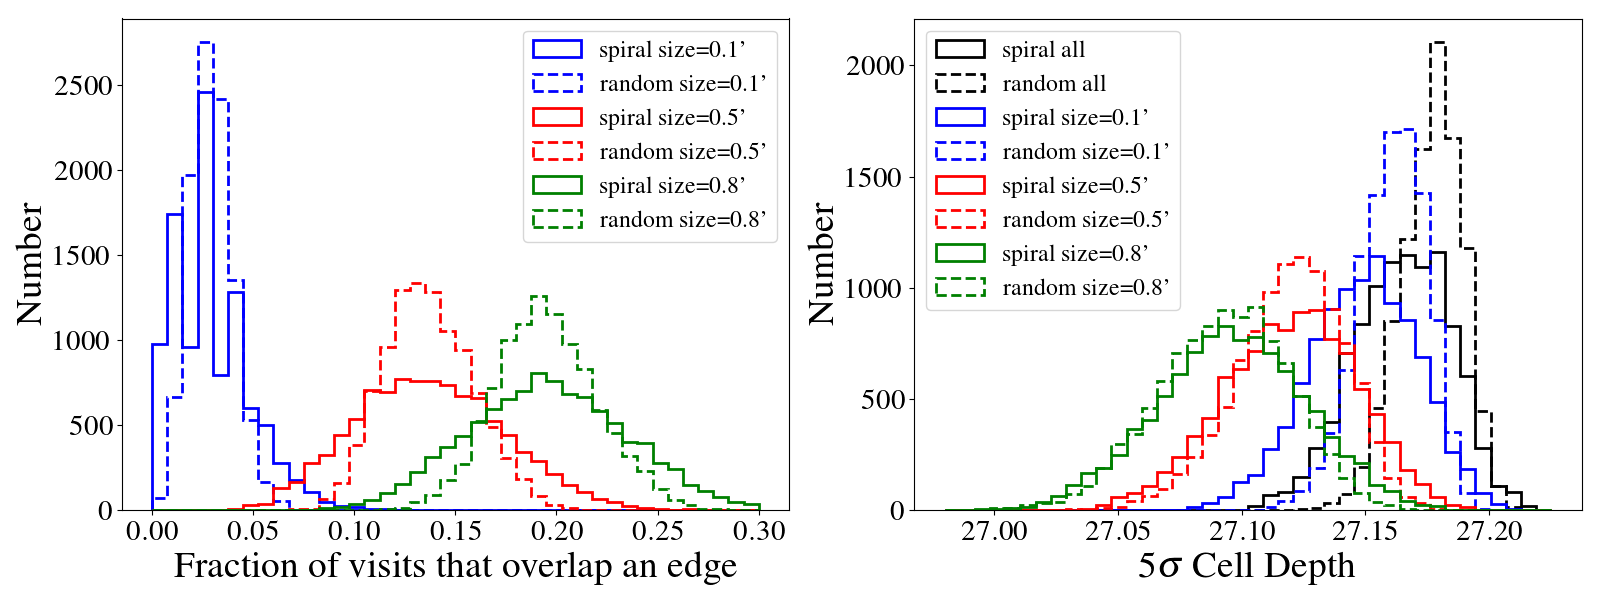
\includegraphics[width=\columnwidth]{cell.png}
\caption{
Left: The fraction of exposures that will need to be rejected for different 
patch sizes and two different dither patterns.  Right:  The corresponding 
distribution of 5$\sigma$ depths for each patch.
}
\label{fig:dither}
%\end{figure*}
\end{figure}

\begin{figure}
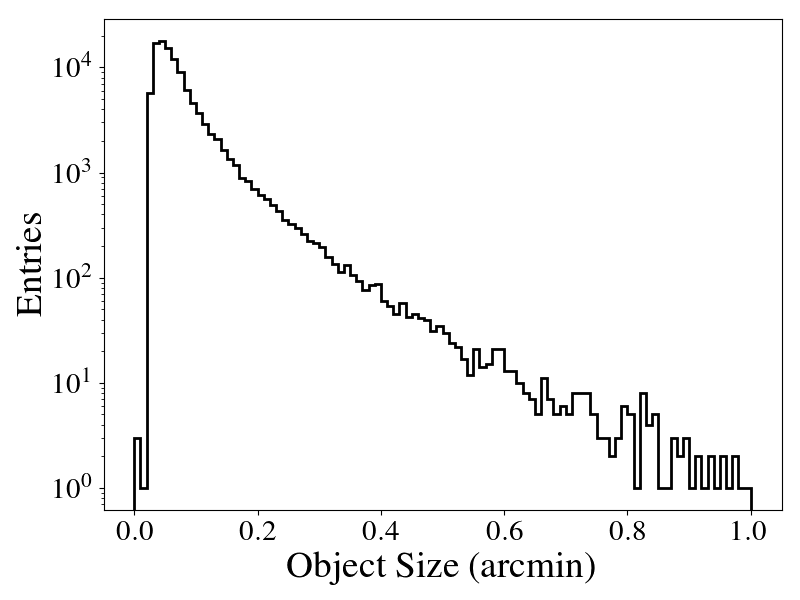
\includegraphics[width=0.5\textwidth]{object_size.png}
\caption{
The distribution of the sizes of blended objects as derived from the HSC 
Ultra-Deep data.
}
\label{fig:size}
\end{figure}

\section{Summary}
\label{Section:Summary}

We have shown that we weak lensing shear can be reliably inferred using coadded
images.  We tested two state-of-the art shear techniques, BFD and \mcal, and in
both cases we detected no additional bias due to coaddition.  We see minimal
loss of loss of information using non-optimal weighted mean coadds for the case
of relatively small PSF size variations (of order ten percent).  The two shear
inference methods are quite different, lending support to the notion that the
use of coadds may be possible for other methods as well.

The key issue for recovering accurate shear is careful handling of the
correlated noise that arises during the coaddition process.  We have explictily
assumed in this study that the coadded noise field is roughly constant over the
size of an object.  The scale of noise variation will depend on the distortion,
warping, etc. which could potentially change for different surveys.

These tests were done on simple inverse variance weighted coadds which are
relatively easy to construct.  However, there are some cases where this
approach may not be optimal.  For example, use such simple coadds will likely
somewhat degrad the ability to classify stars and galaxies, as the width of the
coadded PSF is necessarily larger than that of the best input images.  In this
case there is  clear benfit to constructing optimal coadds.  Exploring this in
more detail is beyond the scope of this work.

We did not address the issue of detecting and characterizing moving objects.
It is likely that some form of multi-epoch fitting will be needed for this.

The cost of applying our approach to real data is that epochs where objects
cross CCD boundaries must be rejected from the coadd, in order to preserve the
continuity of the PSF.  Each object or region of interest must construct a
separate coadd.  These regions of interest must be relatively small to avoid
rejecting too many exposures.  We examined the typical size of blended regions
from the HSC Ultra-Deep field and found that the number of visits we would
reject for a survey like LSST is $< 5\%$.  This results in only a minor loss in
limiting magnitude.  It is not clear however that a multi-epoch fitting
algorithm could fully use these rejected visits as there can be numerous
problems in modeling these galaxies on the edge of a CCD.

XXX Given the shear-dependent detection bias I've recently discovered, it is
likely we will need larger ``coadds in cells'', which will necessarily involve
removing more images.  For Y10 LSST is it possibly these edges are less important?

\bibliographystyle{astroads}
\bibliography{references}

\appendix{S/N}
\section{$S/N$ loss from Coaddition} 
\label{Section:FluxSN}
Here we estimate the additional uncertainty in the measured flux when coadding,
for the example of ``matched-filter'' photometry, where a linear fit is 
performed
for the amplitude of a model.
Let's consider an optimal estimator for a single unknown parameter that is
linear in the observables. Let the model be $A\boldsymbol{m}$, where $A$ is a
scalar amplitude and $\boldsymbol{m}$ is a normalized signal model, or
template. Then the log-likelihood for $A$ (assuming a Gaussian signal
likelihood) and some data vector $\boldsymbol{d}$ is

\begin{align}
\log L = - (\boldsymbol{d} - A\boldsymbol{m})^T\: C^{-1} (\boldsymbol{d} - 
A\boldsymbol{m}) - \frac{1}{2} \det(2\pi C )
\end{align}
where $C$ is the noise covariance.  The optimal estimator $\hat{A}$ is the
value that maximizes this expression for $A$. With some algebra, it can be
shown that this value is:
\begin{align}
\hat{A} = \frac{\boldsymbol{m}^T C^{-1} \boldsymbol{d}}{\boldsymbol{m}^T C^{-1} 
\boldsymbol{m}}
\end{align}
and that the variance of $\hat{A}$ is
\begin{align}
{\rm var}\hat{A} = \frac{1}{{\boldsymbol{m}^T C^{-1} \boldsymbol{m}}}
\end{align}

In the case of photometry, $\boldsymbol{m}$ is the normalized profile of the
star or galaxy, $A$ is the measured flux, and $\boldsymbol{d}$ is the set of
pixels on which the measurement will be made.  The equations above are general,
but for simplicity in what follows, we assume the noise comes from a uniform
background, so there is no signal in the covariance.
For a set of $N$ images of the same sky, the data is the concatenation of the
pixel values in each epoch, i.e., $\boldsymbol{d} = \{d_0, d_1, ..., d_n \}$.
This allows the template $\boldsymbol{m}$ to be the concatenation of the
templates appropriate for each epoch, if for instance the PSF varies from
exposure to exposure.

Now suppose we coadd the images using a straight mean, such that $\langle
\boldsymbol{d} \rangle = \frac{1}{N}\sum\limits_i d_i$, and the covariance
matrix is $C_\coadd = \frac{1}{N^2}\sum\limits_i C_i$.  The template
$\boldsymbol{m}_\coadd$ is then the mean $\boldsymbol{m}_\coadd = 
\frac{1}{N}\sum\limits_i m_i$
and the resulting operation is:

\begin{align}
\hat{A}_\coadd = \frac{\boldsymbol{m}_\coadd^T C_\coadd^{-1} \langle 
\boldsymbol{d} \rangle}{\boldsymbol{m}_\coadd^t 
C_\coadd^{-1}\boldsymbol{m}_\coadd} 
\end{align}
with estimator variance
\begin{align} \label{eq:exact_var_coadd}
{\rm var}\hat{A}_\coadd = \frac{1}{\boldsymbol{m}_\coadd^T 
C_\coadd^{-1}\boldsymbol{m}_\coadd},
\end{align}

where the indices in these expressions run over epochs. The multi-fitting
method, by contrast, would use the optimal estimator for each epoch:

\begin{align}
\hat{A}_{\rm multi} = \frac{\sum\limits_i \boldsymbol{m}_i^T 
C_i^{-1}\boldsymbol{d}_i}{\sum\limits_i \boldsymbol{m}_i^T 
C_i^{-1}\boldsymbol{m}_i}
\end{align}
with estimator variance
\begin{align}
\label{eq:exact_var_multi}
{\rm var}\hat{A}_{\rm multi} = \frac{1}{\sum\limits_i \boldsymbol{m}_i^T 
C_i^{-1}\boldsymbol{m}_i}.
\end{align}

These variance estimators predict, for the case of background-only noise, that 
the variance of the coadd estimator is generally greater than or equal to that of
the optimal estimator using the original images, assuming the templates are
accurate.  This is because the averaged signal will generally be less varied
than the set of input images, such than $\boldsymbol{m}^T C^{-1} \boldsymbol{m}
\sim \sum \boldsymbol{m}^2$ is smaller for the coadd.
In order to gain better intuition for this increased variance, we depart from
generality in the data, and adopt a toy model for the signal.  First, we assume
that the noise in all images is equal, with standard deviation $\eta$, such
that the estimators become

\begin{align}
\hat{A}_{\rm multi} = \frac{\sum\limits_i \boldsymbol{m}_i^T 
\boldsymbol{d}}{\sum\limits_i \boldsymbol{m}_i^T \boldsymbol{m}_i}&, ~~
{\rm var}\hat{A}_{\rm multi} = \frac{\eta^2}{\sum\limits_i 
\boldsymbol{m}_i^T \boldsymbol{m}_i}\\
\hat{A}_\coadd = \frac{\boldsymbol{m}_\coadd^T \langle \boldsymbol{d} 
\rangle}{\boldsymbol{m}_\coadd^T \boldsymbol{m}_\coadd}&, ~~
{\rm var}\hat{A}_\coadd = \frac{\eta^2/N}{\boldsymbol{m}_\coadd^T 
\boldsymbol{m}_\coadd}
\end{align}

We now assume that the template for the coadd is related to that
in the original images by perturbations due to small variations
in a scale of the object $\sigma$:

\begin{align}
\boldsymbol{m}_{\rm i} &= \boldsymbol{m}_\coadd + \Delta \boldsymbol{m}_i \\
&\approx \boldsymbol{m}_\coadd + \frac{\partial 
\boldsymbol{m}_\coadd}{\partial \sigma} \Delta \sigma
\end{align}

The ratio of variances then becomes

\begin{align} \label{eq:generalperturb}
\frac{ {\rm var} \hat{A}_\coadd }{{\rm var} \hat{A}_{\rm multi} } &=  
1 + \frac{1}{N}\frac{\sum\limits_i \Delta \model_i^T \Delta \model_i 
}{\modelc^T \modelc} \\
& \approx 
1 + \frac{(\Delta \sigma)^2}{N}\frac{\sum\limits_i \left( \frac{\partial 
\modelc}{\partial \sigma} \right)_i^T \left( \frac{\partial \modelc}{\partial 
\sigma} \right)_i }{\modelc^T \modelc}
\end{align}

We further assume the template is a round Gaussian

\begin{align}
\modelc = \frac{1}{2 \pi \sigma^2} e^{-r^2/2 \sigma^2 }
\end{align}
with derivative
\begin{align}
\frac{\partial \modelc}{\partial \sigma} &= \frac{1}{2 \pi \sigma^2} 
\frac{2}{\sigma} e^{r^2/2 \sigma^2} \Bigl( \frac{1}{2}\frac{r^2}{\sigma^2} - 1 
\Bigr).
\end{align}

For these gaussian models all terms in equation \ref{eq:generalperturb} can
be readily calculated in the continuous limit, and we find

\begin{align} \label{eq:varbasic}
\left( \frac{ {\rm var} \hat{A}_\coadd }{{\rm var} \hat{A}_{\rm multi} } 
\right)_{\rm toy} = 
1 + 2 \left( \frac{\Delta \sigma}{\sigma} \right)^2
\end{align}

where $(\Delta \sigma)^2$ is to be interpreted as the rms variation of the size.
We expect the increase in variance to be less for the case
of large galaxies convolved by a PSF.  If the galaxy is a round Gaussian with
size $\sigma_g$ and the PSF is a round Gaussian with size $\sigma_p$,
and only the PSF size varies between images,
we can use the chain rule to rewrite equation \ref{eq:varbasic} as

\begin{align} \label{eq:vargal_appendix}
\left( \frac{ {\rm var} \hat{A}_\coadd }{{\rm var} \hat{A}_{\rm multi} } 
\right)_{\rm toy} &= 
1 + 2 \left( \frac{\sigma_p^2}{\sigma_g^2 + \sigma_p^2}\right)^2 \left( 
\frac{\Delta \sigma_p}{\sigma_p} \right)^2 \\
&\equiv 1 + 2 \left( 1 - R \right)^2 \left( \frac{\Delta 
\sigma_p}{\sigma_p} \right)^2
\end{align}

where we have used the definition of the resolution factor $R =
\sigma_g^2/(\sigma_p^2 + \sigma_g^2)$.  This confirms our
intuition that measurements of large galaxies, with $R \sim 1$ will suffer
less increase in variance.
Note that, for this toy model, the template is not exactly equal to the mean of
the individual templates.  Thus we expect the toy model to slightly
over-predict the increase in variance due to coaddition.

\end{document}
